\subsection{Integrais simples}
	\begin{table}[H]
		\centering
		\begin{tabular}{|lclcr|}
			$\integral dx$            & $=$ & $x + c$                       &               &  \\
			$\integral x^p\, dx$      & $=$ & $\dfrac{x^{p + 1}}{p+ 1} + c$ & $\rightarrow$ & $p\neq -1$ \\
			$\integral \e^x\, dx$     & $=$ & $\e^x + c$                    &               &  \\
			$\integral \dfrac{dx}{x}$ & $=$ & $\ln|x| + c$                  &               &  \\
			$\integral u^p\, du$      & $=$ & $\dfrac{u^{p + 1}}{p+ 1} + c$ & $\rightarrow$ & $p\neq -1$ \\
			$\integral \e^u\, du$     & $=$ & $\e^u + c$                    &               &  \\
			$\integral \dfrac{du}{u}$ & $=$ & $\ln|u| + c$                  &               &  \\
			$\integral p^u\, du$      & $=$ & $\dfrac{p^u}{\ln|p|} + c$     &               &
		\end{tabular}
		\caption{Integrais simples}
		\label{integrais_simples}
	\end{table}

\subsection{Integrais trigonométricas}
	\begin{table}[H]
		\centering
		\begin{tabular}{|lcl|}
			$\integral \sen(u)du$                      & $=$ & $-\cos(u) + c$                   \\
			$\integral \cos(u)du$                      & $=$ & $\sen(u) + c$                    \\
			$\integral \tg(u)du$                       & $=$ & $\ln|\sec(u)| + c$               \\
			$\integral \cotg(u)du$                     & $=$ & $\ln|\sen(u)| + c$               \\
			$\integral \sec(u)du$                      & $=$ & $\ln|\sec(u) + \tg(u)| + c$      \\
			$\integral \cossec(u)du$                   & $=$ & $\ln|\cossec(u) - \cotg(u)| + c$ \\
			$\integral \sec^2(u)du$                    & $=$ & $\tg(u) + c$                     \\
			$\integral \cossec^2(u)du$                 & $=$ & $-\cotg(u) + c$                  \\
			$\integral \sec(u)\tg(u)du$                & $=$ & $\sec(u) + c$                    \\
			$\integral \cossec(u)\cotg(u)du$           & $=$ & $-\cossec(u) + c$                \\
			$\integral \dfrac{du}{\sqrt{1 - x^2}}$     & $=$ & $\arcsen(x) + c$                 \\
			$-\integral \dfrac{du}{\sqrt{1 - x^2}}$    & $=$ & $\arccos(x) + c$                 \\
			$\integral \dfrac{du}{1 + x^2}$            & $=$ & $\arctg(x) + c$                  \\
			$-\integral \dfrac{du}{1 + x^2}$           & $=$ & $\arccotg(x) + c$                \\
			$\integral \dfrac{du}{|x|\sqrt{x^2 - 1}}$  & $=$ & $\arcsec(x) + c$                 \\
			$-\integral \dfrac{du}{|x|\sqrt{x^2 - 1}}$ & $=$ & $\arccossec(x) + c$
		\end{tabular}
		\caption{Integrais trigonométricas}
		\label{integrais_trigonometricas}
	\end{table}

\subsection{Relação entre coordenada cartesina e polar}
	\begin{figure}[H]
		\centering
		\subfloat[Coordenada cartesiana ou retangular]{
			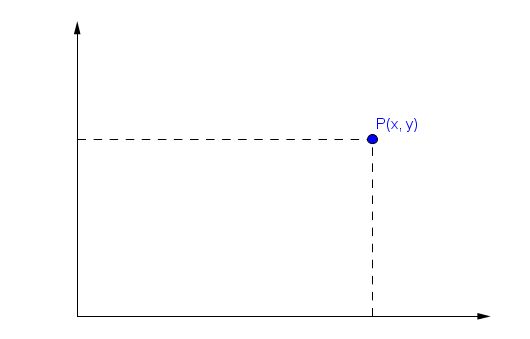
\includegraphics[width=0.29\paperwidth]{coordenada_cartesiana.png}
		}
		\quad\quad
		\subfloat[Coordenada polar]{
			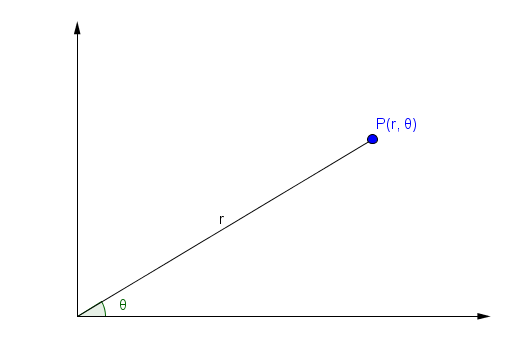
\includegraphics[width=0.29\paperwidth]{coordenada_polar.png}
		}
		
		\caption{Coordenada cartesina e polar}
		\label{coordenada_cartesiana_polar}
	\end{figure}
	
	$$P(x,y) \rightarrow P(r,\theta)$$
	
	\begin{table}[H]
		\centering
		\begin{tabular}{|lclcl|}
			     &     & $x$                                 & $=$ & $r\,\cos \theta$                                                         \\
			     &     & $y$                                 & $=$ & $r\,\sen \theta$                                                         \\
			     &     & $x^2 + y^2$                         & $=$ & $r^2$                                                                    \\
			$da$ & $=$ & $dxdy$                              & $=$ & $r\,drd\theta$                                                           \\
			$v$  & $=$ & $\iintegral_{R(x,y)} f(x,y)\, dxdy$ & $=$ & $\iintegral_{R(r,\theta)} f(r\,\cos \theta,r\,\sen \theta) r\,drd\theta$
		\end{tabular}
		\caption{Relação entre coordenada cartesina e polar}
		\label{relacao_coordenada_cartesiana_polar}
	\end{table}